%!TEX root = index.tex
\chapter{Analises}
\label{cha:analises}

\section{Samsung}

A partir de conversas com Luís Guilherme Selber, responsável pela operação do Laboratório Ocean, obtivemos a seguinte análise:

\begin{figure}[H]
\caption{Análise do Ocean - Samsung}
\centerline{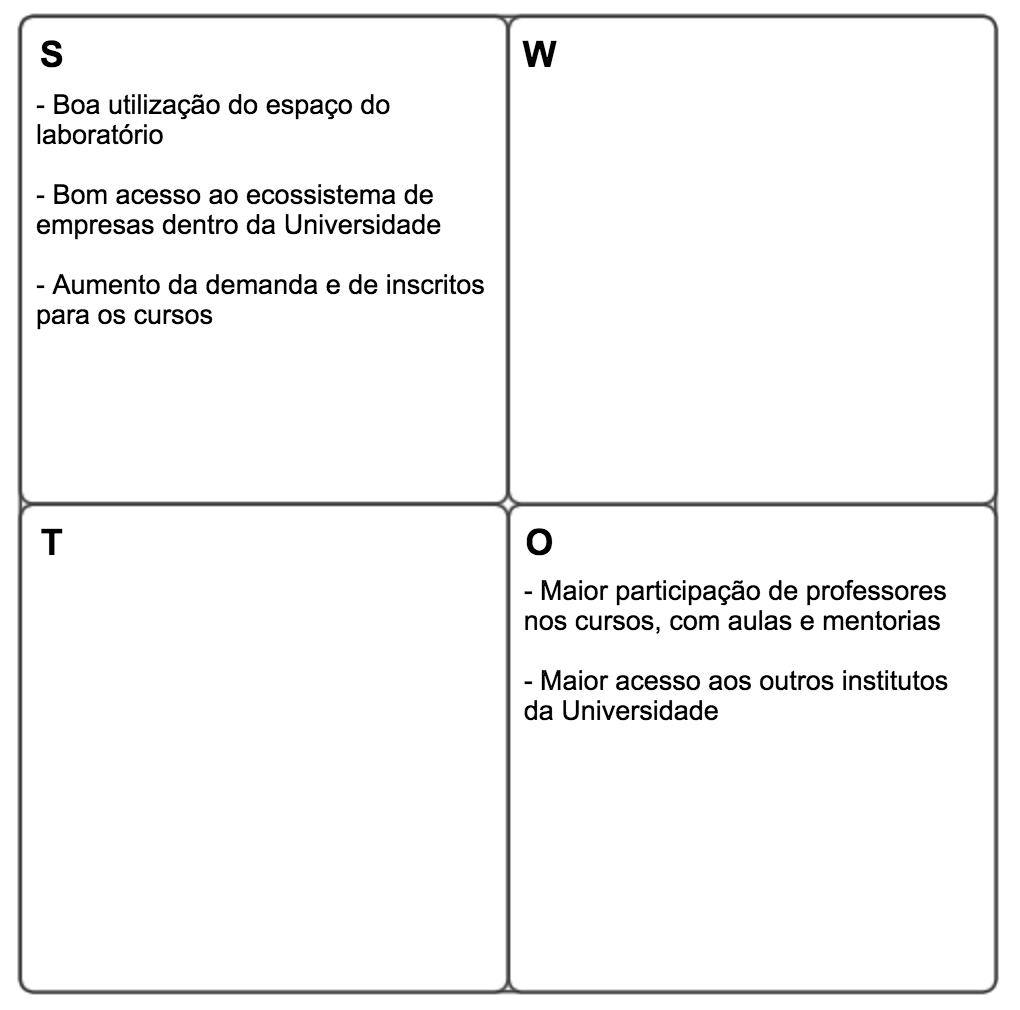
\includegraphics[scale=0.75]{img/samsungswot}}
\label{fig:swotsamsung}
\caption* {Fonte: Elaborado pelo próprio autor}
\end{figure}

A ausência de fraquezas e ameaças se dá - segundo o entrevistado - pelo fato de o projeto estar em uma fase inicial. Não há formalidades estabelecidas como reuniões periódicas, quando é necessário conversar sobre algo é fácil encontrar um professor no corredor ou em sua sala, portanto as interações se limitam às necessidades de um ou outro, sem conflitos até o momento. A própria gestão de uso do Laboratório para as atividades de cada instituição não gera conflitos pois as necessidades de uso do laboratório por cada parte já foram claramente estabelecidas nas reuniões iniciais de fechamento do projeto.

Em relação aos pontos fortes, destaca-se o fato de o laboratório sofrer uma mudança muito positiva devido à mudança de localidade para dentro da universidade. A presença do laboratório dentro do PRO mudou completamente a utilização do laboratório, que agora é ocupado das 08 da manhã até as 22 da noite de segunda a sexta, fato que não acontecia na Faria Lima. Quando na Av. Brigadeiro Faria Lima, a Samsung exercia um papel ativo de sediar eventos próprios ou externos com o intuito de divulgar e preencher o espaço do laboratório. Tudo isso porque mais pessoas utilizando o espaço ajuda a divulgar mais o programa e os cursos oferecidos pelo laboratório. Não obstante, além dos próprios cursos dados pelo laboratório, ainda existe um custo com equipamentos e internet que não deveria existir em vão.

Outra grande vantagem de estar dentro da universidade consiste no fato de a USP ser um ecossistema de parcerias com diversas empresas. Dentro desse meio, a Samsung ganha expande sua rede de contatos com outras empresas, já tendo provido até o momento reuniões com outras grandes empresas do mercado nacional.

O último ponto forte mencionado foi o aumento de demanda pelos cursos básicos e intensivos, houve um grande aumento principalmente por alunos da universidade. A proximidade com o NEU e a POLI permite uma divulgação muito mais fácil do laboratório na universidade.

Em relação às oportunidades, a Samsung vê como maiores oportunidades de melhoria uma maior participação de professores nos cursos do laboratório, seja através de aulas ou mentorias. Acredita-se que exista uma sinergia muito bom entre a academia e empresa no sentido de prender a atenção e incentivar os alunos dos cursos a buscarem mais conhecimento nas suas áreas de interesse.

Também acredita-se que possa haver uma adesão maior aos cursos e ao próprio dia a dia do laboratório por parte de outras instituições da Universidade. Tanto a FEA quanto o IME por suas formações ligadas ao empreendedorismo e ao desenvolvimento mostram ser muito compatíveis com os programas oferecidos pelo Ocean, entretanto a grande maioria de adeptos vêm da Escola Politécnica.

\section{PRO}

\begin{figure}[H]
\caption{Análise do Ocean - PRO}
\centerline{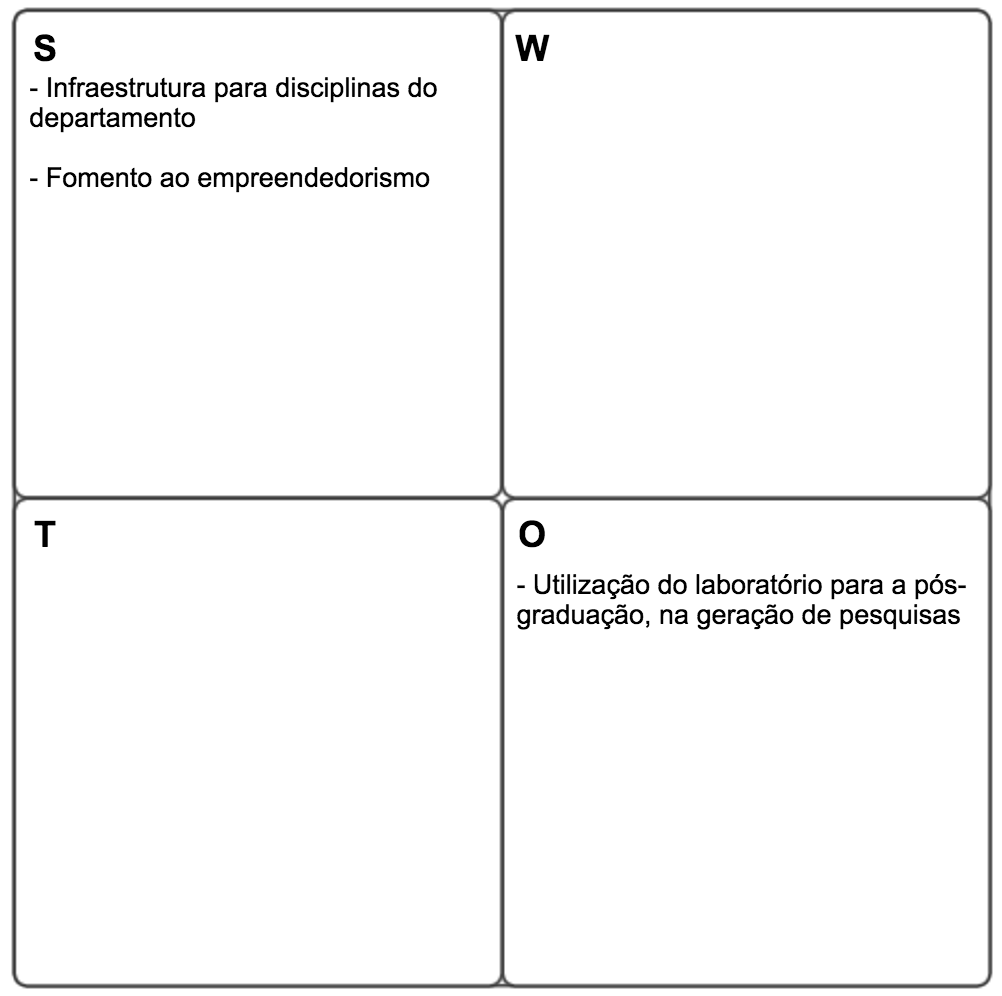
\includegraphics[scale=0.75]{img/proswot}}
\label{fig:swotpro}
\caption* {Fonte: Elaborado pelo próprio autor}
\end{figure}

Em uma primeira instância, a parceria com o Ocean é avaliada como um investimento externo aplicado ao departamento e à universidade, e como uma oportunidade que surgiu e foi executada com muita rapidez. Entre as conversas iniciais e o final da reforma da área do laboratório foram cerca de 4 meses.

Dado esse investimento, a discussão se dá em como reverter esse investimento para pesquisa, ensino e extensão baseado nas propostas do laboratório. Segundo o PRO, já houve um impacto bastante positivo no ensino, pois a estrutura do laboratório tira o gargalo anteriormente existente das máquinas e espaço físico para a docência de várias disciplinas do departamento.

Entretanto como ainda está em fase inicial, não houve tempo para os pós-graduandos começarem a utilizar o espaço e iniciar as pesquisas, sendo essa a maior oportunidade de desenvolvimento do laboratório, que acontecerá inevitavelmente.

\section{NEU}

\begin{figure}[H]
\caption{Análise do Ocean - NEU}
\centerline{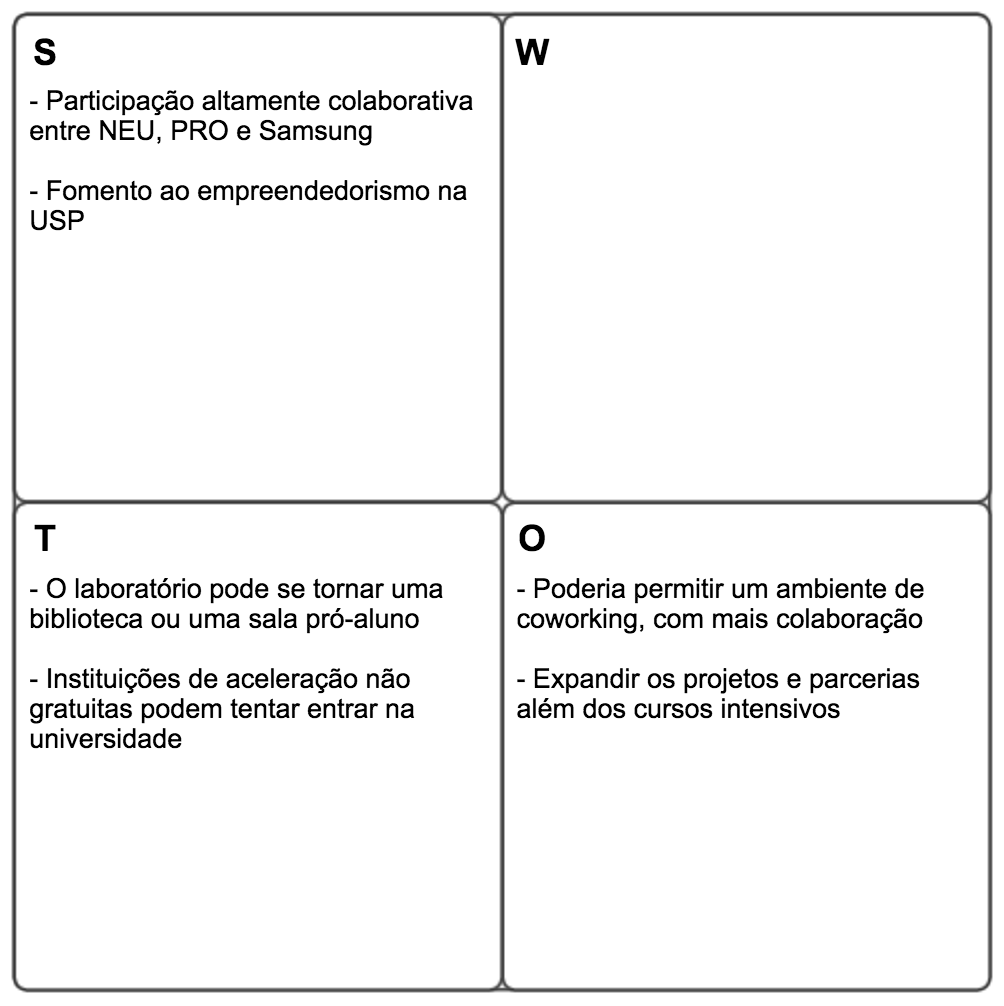
\includegraphics[scale=0.75]{img/neuswot}}
\label{fig:swotneu}
\caption* {Fonte: Elaborado pelo próprio autor}
\end{figure}

Segundo Juliana Uechi, atual responsável pelo funcionamento do NEU, a presença do Ocean por si só já contribui com o fomento à cultura de empreendedorismo dentro da Universidade, principal objetivo do NEU. Isso porque ainda existe uma carência de motivação pelo empreendedorismo, ainda mais em tempos de crise, a qual encontra no Ocean uma ferramenta gratuita com suporte à pré-aceleração de empresas. 

Atualmente existe uma colaboração ativa entre NEU, PRO e Samsung, principalmente em relação ao atual módulo de curso intensivo do laboratório, que envolve participação de todas as partes. De forma geral, a Samsung é responsável pelo acompanhamento do programa e pela capacitação, e o NEU e o PRO utilizam de suas conexões para trazer mentores às empresas participantes, normalmente ex-alunos que abriram as próprias empresas. Tais colaborações poderiam, segundo Juliana, ir além da participação nos cursos intensivos, porém a agenda de ambas as instituições encontra-se lotada

Em relação à infraestrutura do laboratório, o NEU acredita que o uso do laboratório é subutilizado quando cursos não estão acontecendo. O cenário atual de funcionamento é similar ao de uma biblioteca ou uma sala pró-aluno, onde alunos vão com tarefas individuais ou materiais de estudo, o que é de certa forma redundante pois já há uma biblioteca no departamento. Como uma frente de desenvolvimento e empreendedorismo, poderia haver mais espaço para \textit{coworking} e atividades colaborativas dentro do laboratório. Que fosse uma sala que gerasse valor através da discussão, não da absorção individual, que é igualmente importante, mas a biblioteca seria uma lugar mais adequado para esse tipo de atividade.

Por fim, é ressaltado a sinergia entre empresas que colaboram com o fomento à cultura de empreendedorismo, considerando que por mais que compartilhem o relacionamento com \textit{startups} via pré-aceleração, os alunos precisam ser motivados através de métodos diferentes. E pensando sempre no aluno e nas suas futuras empresas, um ambiente com diversas instituições de fomento ao empreendedorismo e aceleração, evita a entrada na universidade de instituições não-gratuitas, seja através de inscrição nos cursos ou via equity das empresas.

\section{Alunos}

\begin{figure}[H]
\caption{Análise do Ocean - Alunos}
\centerline{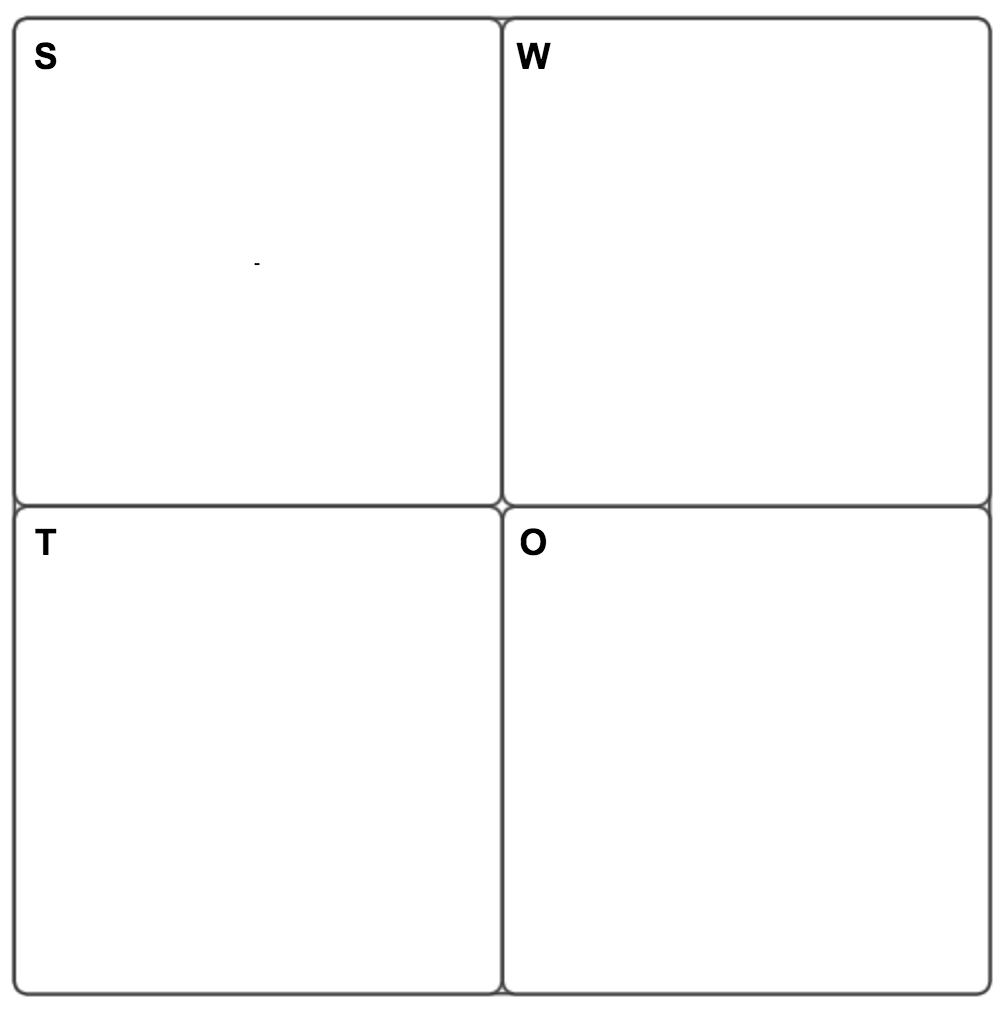
\includegraphics[scale=0.75]{img/generalswot}}
\label{fig:swotalunos}
\caption* {Fonte: Elaborado pelo próprio autor}
\end{figure}

\section{Cursistas}

A análise dos cursistas é segmentada devido aos dois tipos de cursos dados pelo laboratório e o tipo de material a ser analisado para cada. Para os alunos de cursos básicos, foi utilizada a metodologia de \citeonline{bardin} para analisar os questionários de respostas, ao passo que com os alunos de cursos intensivos foram realizadas entrevistas semi-estruturadas.

\subsection{Cursos Básicos}

Em relação aos cursistas dos cursos básicos, utilizamos o software já mencionado para mapear as palavras com maior recorrência nas respostas dos questionários para cursos básicos, para as seguintes perguntas:

\begin{itemize}
\item O que mais o motivou nesse curso?
\item O que você acha que pode ser melhorado?
\item Qual tema você gostaria que fosse abordado num próximo curso?
\end{itemize}

Como forma de simplificação, utilizaremos como nomenclatura de cada questão os termos 'motivação', 'melhorias' e 'novidades', respectivamente. Em seguida, foi aplicada a metodologia de \citeonline{bardin} para as respostas de cada uma.

\subsubsection*{Pré-exploração do material}

A pré-exploração segue o mesmo modelo para todas as questões, devido aos seguintes motivos:

\begin{description}
\item[Modelo único de coleta] O instrumento de coleta de dados utilizado nas pesquisas foi o mesmo questionário reutilizado nos últimos 2 anos. Dado que no momento de preenchimento os cursistas acabaram de realizar os cursos, a percepção deles diante do conteúdo passado está bem fresca, e a contribuição também acaba sendo maior com uma taxa maior de respostas. Isso permitiu que o autor minimizasse a possibilidade de encontrar poucos dados ou dados inconsistentes com a realidade apresentada no curso.
\item[Perguntas sequenciais com o mesmo formato] As perguntas qualitativas no final do questionário são bastante diretas e fáceis de serem respondidas. O objetivo de cada questão pode ser traduzido pela própria nomenclatura previamente estabelecida: identificar a motivação dos cursistas que optaram por 'gastar' cerca de 3 horas em um curso de capacitação, identificar melhorias dentro do próprio curso para melhorar a sua qualidade de forma geral, e estar sempre atualizado para identificar a sinergia entre esse curso e outros temas de interesse dos cursistas. O formato das perguntas permitiu uma análise não exaustiva de dados pois as respostas apresentavam algumas poucas linhas, e a informação presente é suficiente para atender as necessidades da Samsung.
\item[Respostas consolidadas em um mesmo lugar] Todas as respostas foram consolidadas em planilhas digitais, de tal forma que cada resposta corresponde a uma linha, e cada pergunta é uma coluna. Esse formato simplificou a leitura flutuante realizada sobre as respostas, pois um simples \textit{scroll} na tela já traz um novo set de respostas, sem haver muito desgaste mental do autor.
\end{description}

Conforme foi ressaltado, a leitura flutuante foi o principal elemento da pré-exploração do material, pois permitiu identificar o tamanho das respostas (curtas), a variedade das respostas (baixa) e a consequente pré-aprovação da possibilidade de analisá-las e categorizá-las posteriormente. Embora sejam só características relativas observas pelo autor, elas representam a inferência ilustrada por \citeonline{bardin} como pontos de partida ou hipóteses para as próximas etapas.

\subsubsection*{Definição das unidades de análise}

Embora o autor já tivesse ideia da convergência das respostas para certos temas devido às observações obtidas na fase de pré-exploração, não saberia ainda descrever quais seriam os temas principais, e muito menos quantificá-los por número de incidências. Portanto, de forma a tentar atribuir as principais categorias, foi decidido analisar o número de incidências de cada palavra em todas as respostas, por se tratarem de textos curtos e informais.

Após uma análise inicial, observou-se que muitas palavras tinham sinergia entre si e apresentavam-se dentro de um mesmo contexto. Portanto também foram mapeadas todas as palavras que aparecem em uma mesma frase que outro palavra. Dessa forma é possível observar as palavras que aparecem em um mesmo contexto, e logo, possuem bastante sinergia entre si.

Foi considerado como premissa que todas as palavras de cada resposta não se repetem na mesma resposta - com exceção de palavras auxiliares, como artigos e pronomes - de tal forma que seria possível atribuir a linha de origem de cada palavra sem repetições.

\subsubsection*{Tratamento dos dados}

De forma a configurar o software a trabalhar em cima das respostas, foi feita uma extração dos dados da planilha no software \textit{Numbers} em um MacBook para o formato CSV, que é um arquivo de texto puro com quebras de linha e separação por vírgulas. Como o arquivo original, cada linha corresponde a uma resposta e cada elemento entre vírgulas corresponde a uma pergunta. Portanto para cada pergunta a ser analisada, são percorridas todas as linhas e só analisados os elementos correspondentes.

Por se tratarem de todas as palavras da língua portuguesa, foi feito um trabalho manual e iterativo de descartar todas as palavras que não agregariam valor semântico esperado à frase, como pronomes, artigos, verbos auxiliares, conjunções e preposições. Foi uma opção não realizar uma integração com algum software ou \textit{Web API} de Língua Portuguesa pela necessidade e esforço em garantir a confiabilidade do mesmo, portanto a partir do próprio conhecimento do idioma foram feitas iterações e remoções de palavras indesejadas.

Também foram eliminadas as palavras relativas à 'curso' e 'aula', pois todas as perguntas são direcionadas a como melhorar, motivar ou trazer novas coisas para o curso e para a aula, portanto foram consideradas redundantes para a análise.

Outro tratamento realizado foi a remoção de espaços em excesso, pontuações e o emprego das aspas, pois estes atrapalhavam a contagem de palavras.

A partir dos tratamentos descritos e de outros específicos a cada questão, foi possível elaborar uma tabela como \textit{output} do software utilizado. A tabela representa uma contagem das principais palavras presentes nas respostas, acompanhadas de outras que aparecem em um mesmo contexto, e de um exemplo de respostas para ilustrar o uso das palavras de forma conjunta. O exemplo é obtido randomicamente através de uma busca por respostas que apresentem ambas as palavras. Para isso, foram adotadas algumas constantes para aplicação no software:

\begin{itemize}
\item Número mínimo de incidências para ser considerado na tabela: 1\% do número de respostas
\item Número de palavras com sinergia que são exibidas: 3
\end{itemize}

Esses números foram definidos posteriormente, pois foram feitos alguns testes para identificar até onde poderia ser filtrado os dados para não perder nenhuma informação relevante. Essas constantes se apresentaram boas tanto de forma ilustrativa para o trabalho quanto para a categorização posteriormente feita das palavras.

\subsubsection*{Tratamento dos dados: \textit{Motivação}}

Novamente, como não há integração com um dicionário de Língua Portuguesa, foi possível de fazer agrupamentos de palavras qeu se encontravam em um mesmo contexto, comprovado pelas sinergia com as mesmas palavras ou similares. 

Foi possível agrupar posteriormente palavras que se apresentavam em diferentes flexões gramaticais de número, como: 

\begin{itemize}
\item 'conhecimento' e 'conhecimentos'
\item 'tecnologia' e 'tecnologias' 
\item 'novas' e 'nova' 
\item 'ferramenta' e 'ferramentas' 
\item 'novos' e 'novo' 
\item 'apps' e 'app'
\item 'aplicativos' e 'aplicativo'
\end{itemize}

Também foram agrupadas palavras com flexões gramaticais de gênero:

\begin{itemize}
\item 'novas' e 'novos'
\end{itemize}

Por fim, palavras com mesmo nível semântico:

\begin{itemize}
\item 'app' e 'aplicativo'
\item 'instrutor' e 'professor'
\end{itemize}

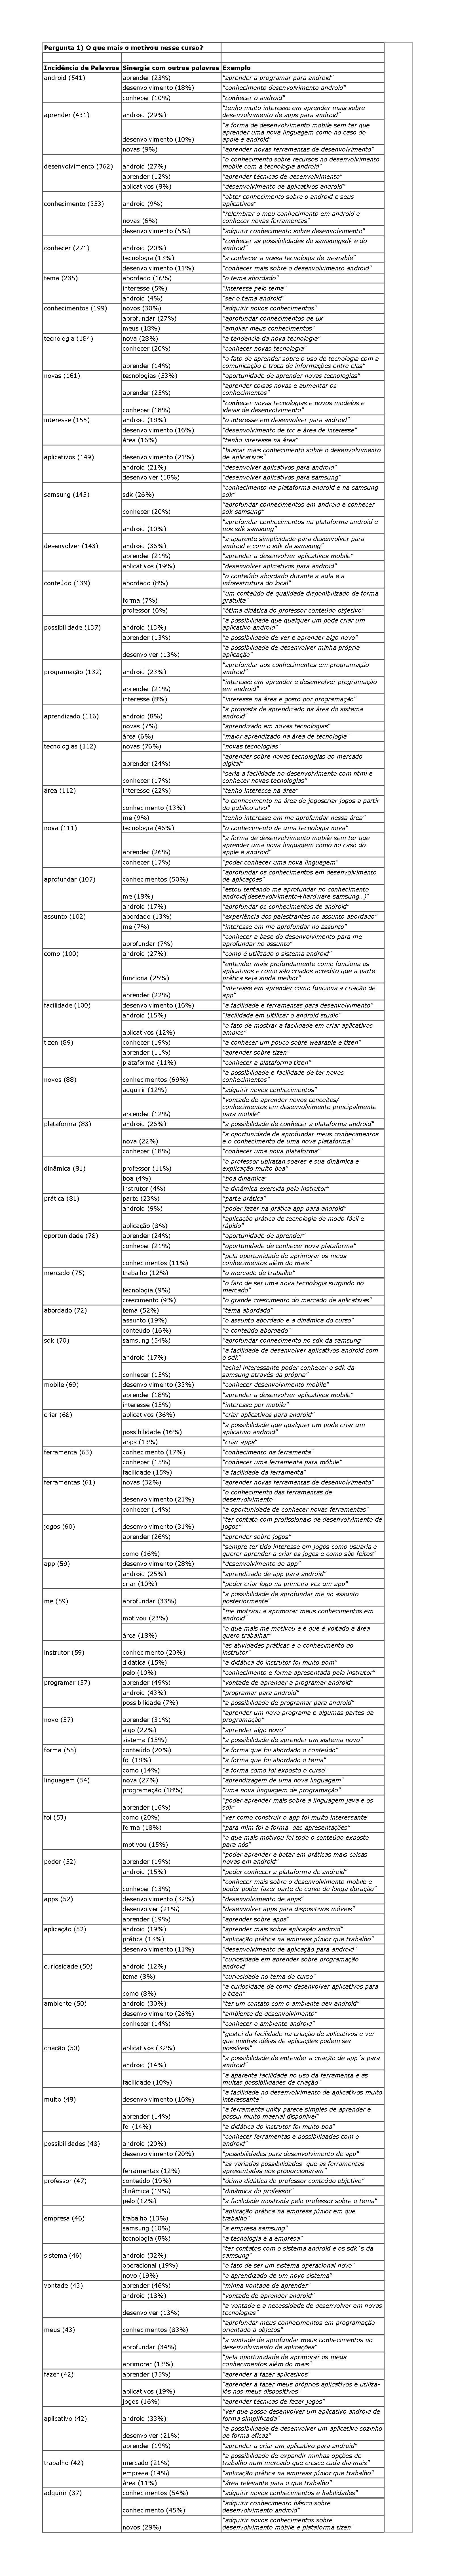
\includepdf[pages=-, pagecommand={}]{Pergunta1.pdf}

\subsubsection*{Categorização e sub-categorização - \textit{Motivação}}

Após analisar a incidência de palavras, foi possível observar a partir dos exemplos uma ambiguidade promovidos pela pergunta em questão. A interpretação correta dessa pergunta seria "quais foram os pontos do curso que você achou mais interessante / relevante?", porém a maior parte das respostas aparentemente a interpretou como "o que o motivou a fazer o curso?". Isso gerou uma séria de respostas relacionadas ao próprio tema do curso, como "interesse por desenvolvimento android e SDK da samsung". Dado que o tem mais recorrente de apresentação do curso chama-se "Introdução ao Desenvolvimento de Aplicativos Android \& Samsung SDK", acaba-se por ter respostas redundantes. Também ocorreram respostas inerentes ao contexto de mercado de trabalho envolvendo programação, o que também foge do objetivo proposto por essa pergunta. Foi passado para a Samsung uma proposta de reformulação dessa pergunta, baseada em como deseja-se utilizar essa informação posteriormente.

Entretanto, ainda foi possível extrair algumas informações a respeito de pontos elogiados do curso, como:

\begin{itemize}
\item A ocorrência de 'professor' e 'dinâmica' indicaram a aceitação pelos alunos do modelo proposto pelo curso, e elencaram estes como um fator motivador.
\item A palavra 'prática' indica que os alunos gostaram da parte prática dos cursos, que indiretamente deve contribuir com a dinâmica elogiada no item anterior.
\end{itemize}

\subsubsection*{Tratamento dos dados: \textit{Melhorias}}

Em relação à flexão gramatical de número e gênero e semântica, foram agrupadas as seguintes palavras

\begin{itemize}
\item 'práticas', 'práticos', 'prático' e 'prática'
\item 'professor', 'instrutor', 'instrutores' e 'professores'
\item 'conhecimento' e 'conhecimentos'
\item 'app', 'apps', 'aplicativo' e 'aplicativos'
\end{itemize}

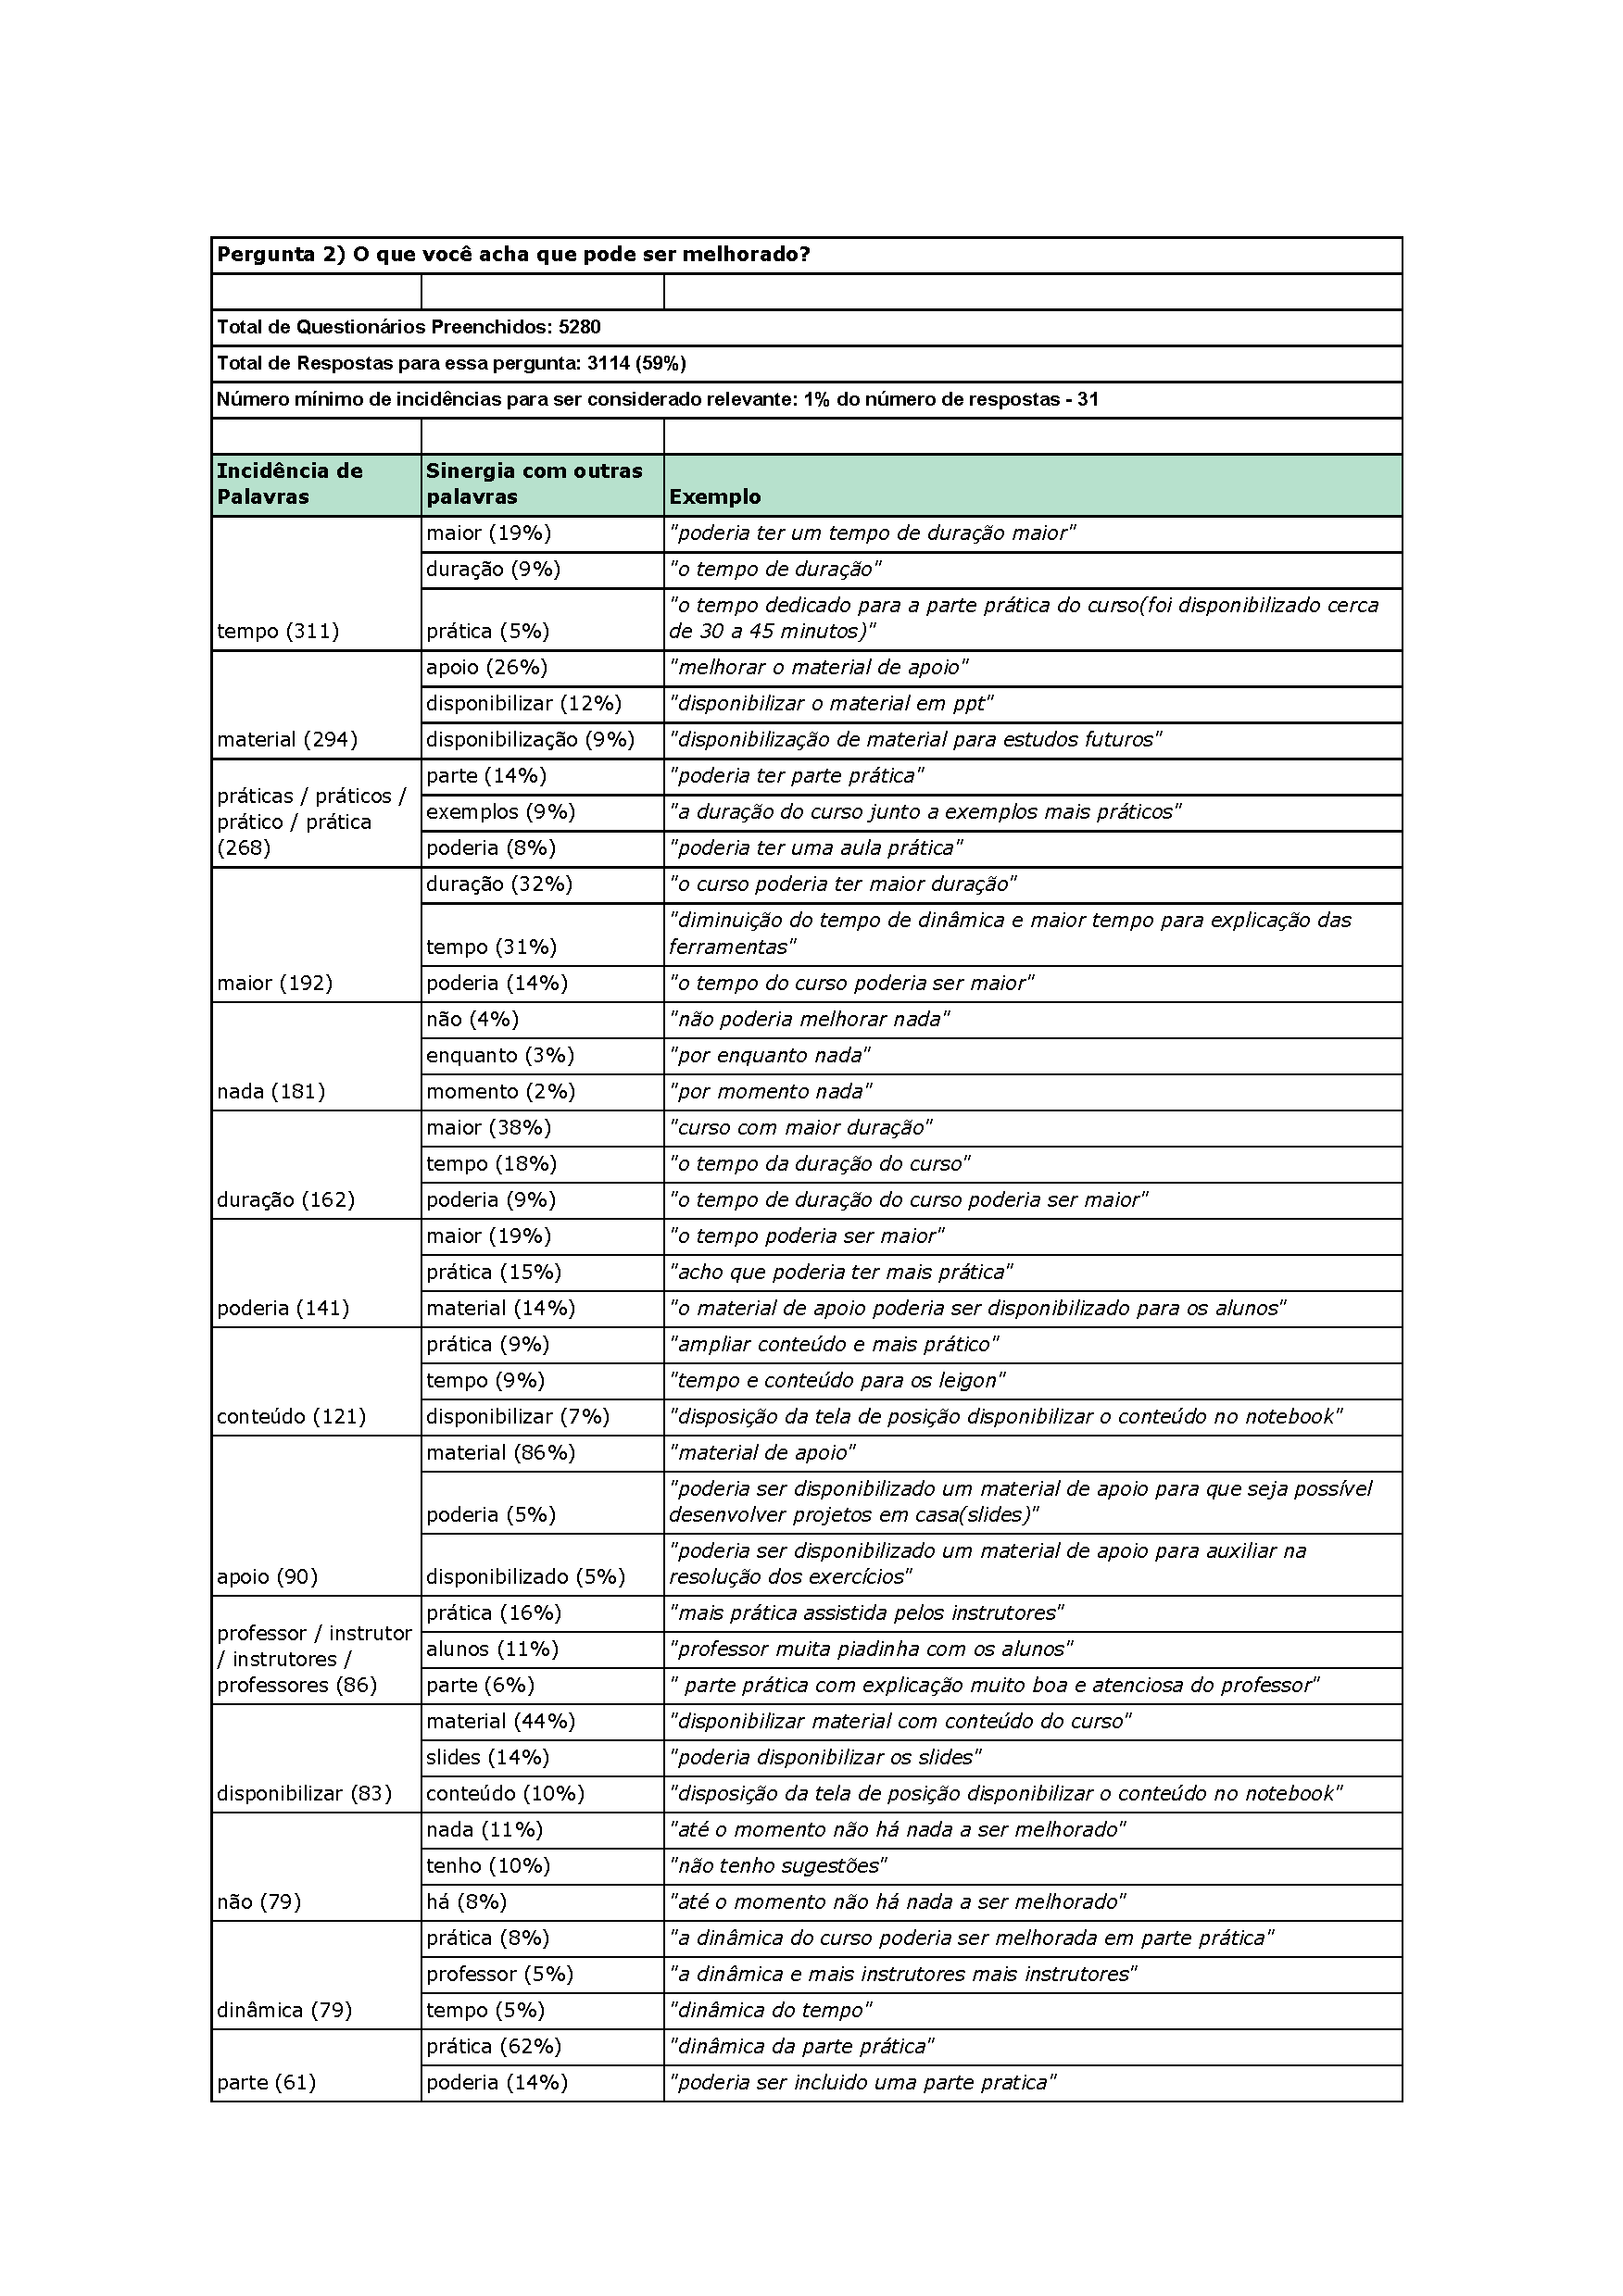
\includepdf[pages=-, pagecommand={}]{Pergunta2.pdf}

\subsubsection*{Categorização e sub-categorização - \textit{Melhorias}}

Diferentemente da questão anterior, esse item é compreendido muito melhor pelos alunos, e as respostas tornam-se muito mais objetivas. A recorrência já mostra de imediato três pontos a serem melhorados, a duração do curso, problemas com o material de apoio e a inclusão de mais modalidades práticas dentro da aula. Esses problemas, de forma conjunta, correspondem a cerca de 40\% das respostas analisadas.

A duração do curso se mostra um grande problema, se mostrando incidente através das palavras 'tempo', 'duração' e 'carga horária', essa última com as duas palavras aparecendo na tabela.

Os problemas com o material de apoio também se mostra recorrente através da expressão 'material de apoio', 'conteúdo', 'slides', 'slides' e 'apresentação'. A maior parte se associa com as palavras 'disponibilizar' e 'disponibilização', indicando que o material utilizado não é entregue para os alunos.

A recorrência de termos ligados à prática indica que há uma necessidade de aumentar a parte prática no programa diante da teórica. Aliada essa informação à questão da carga horária, deve ser desejável que se for possível aumentar o tempo de curso, que ele aumenta em termos práticos e não teóricos.

Em menor volume (menos de 5\% cada), aparecem questões como maior flexibilização do horário ou disponibilidade de horários, através das palavra 'horário' e 'dias', e problemas com equipamentos no laboratório.

\subsubsection*{Tratamento dos dados: \textit{Novidades}}

Em relação à flexão gramatical de número e gênero e semântica, foram agrupadas as seguintes palavras

\begin{itemize}
\item 'jogos', 'jogo', 'game' e 'games'
\item 'aprofundar' e 'aprofundamento'
\item 'práticas', 'práticos', 'prático' e 'prática'
\item 'app', 'apps', 'aplicativo' e 'aplicativos'
\end{itemize}

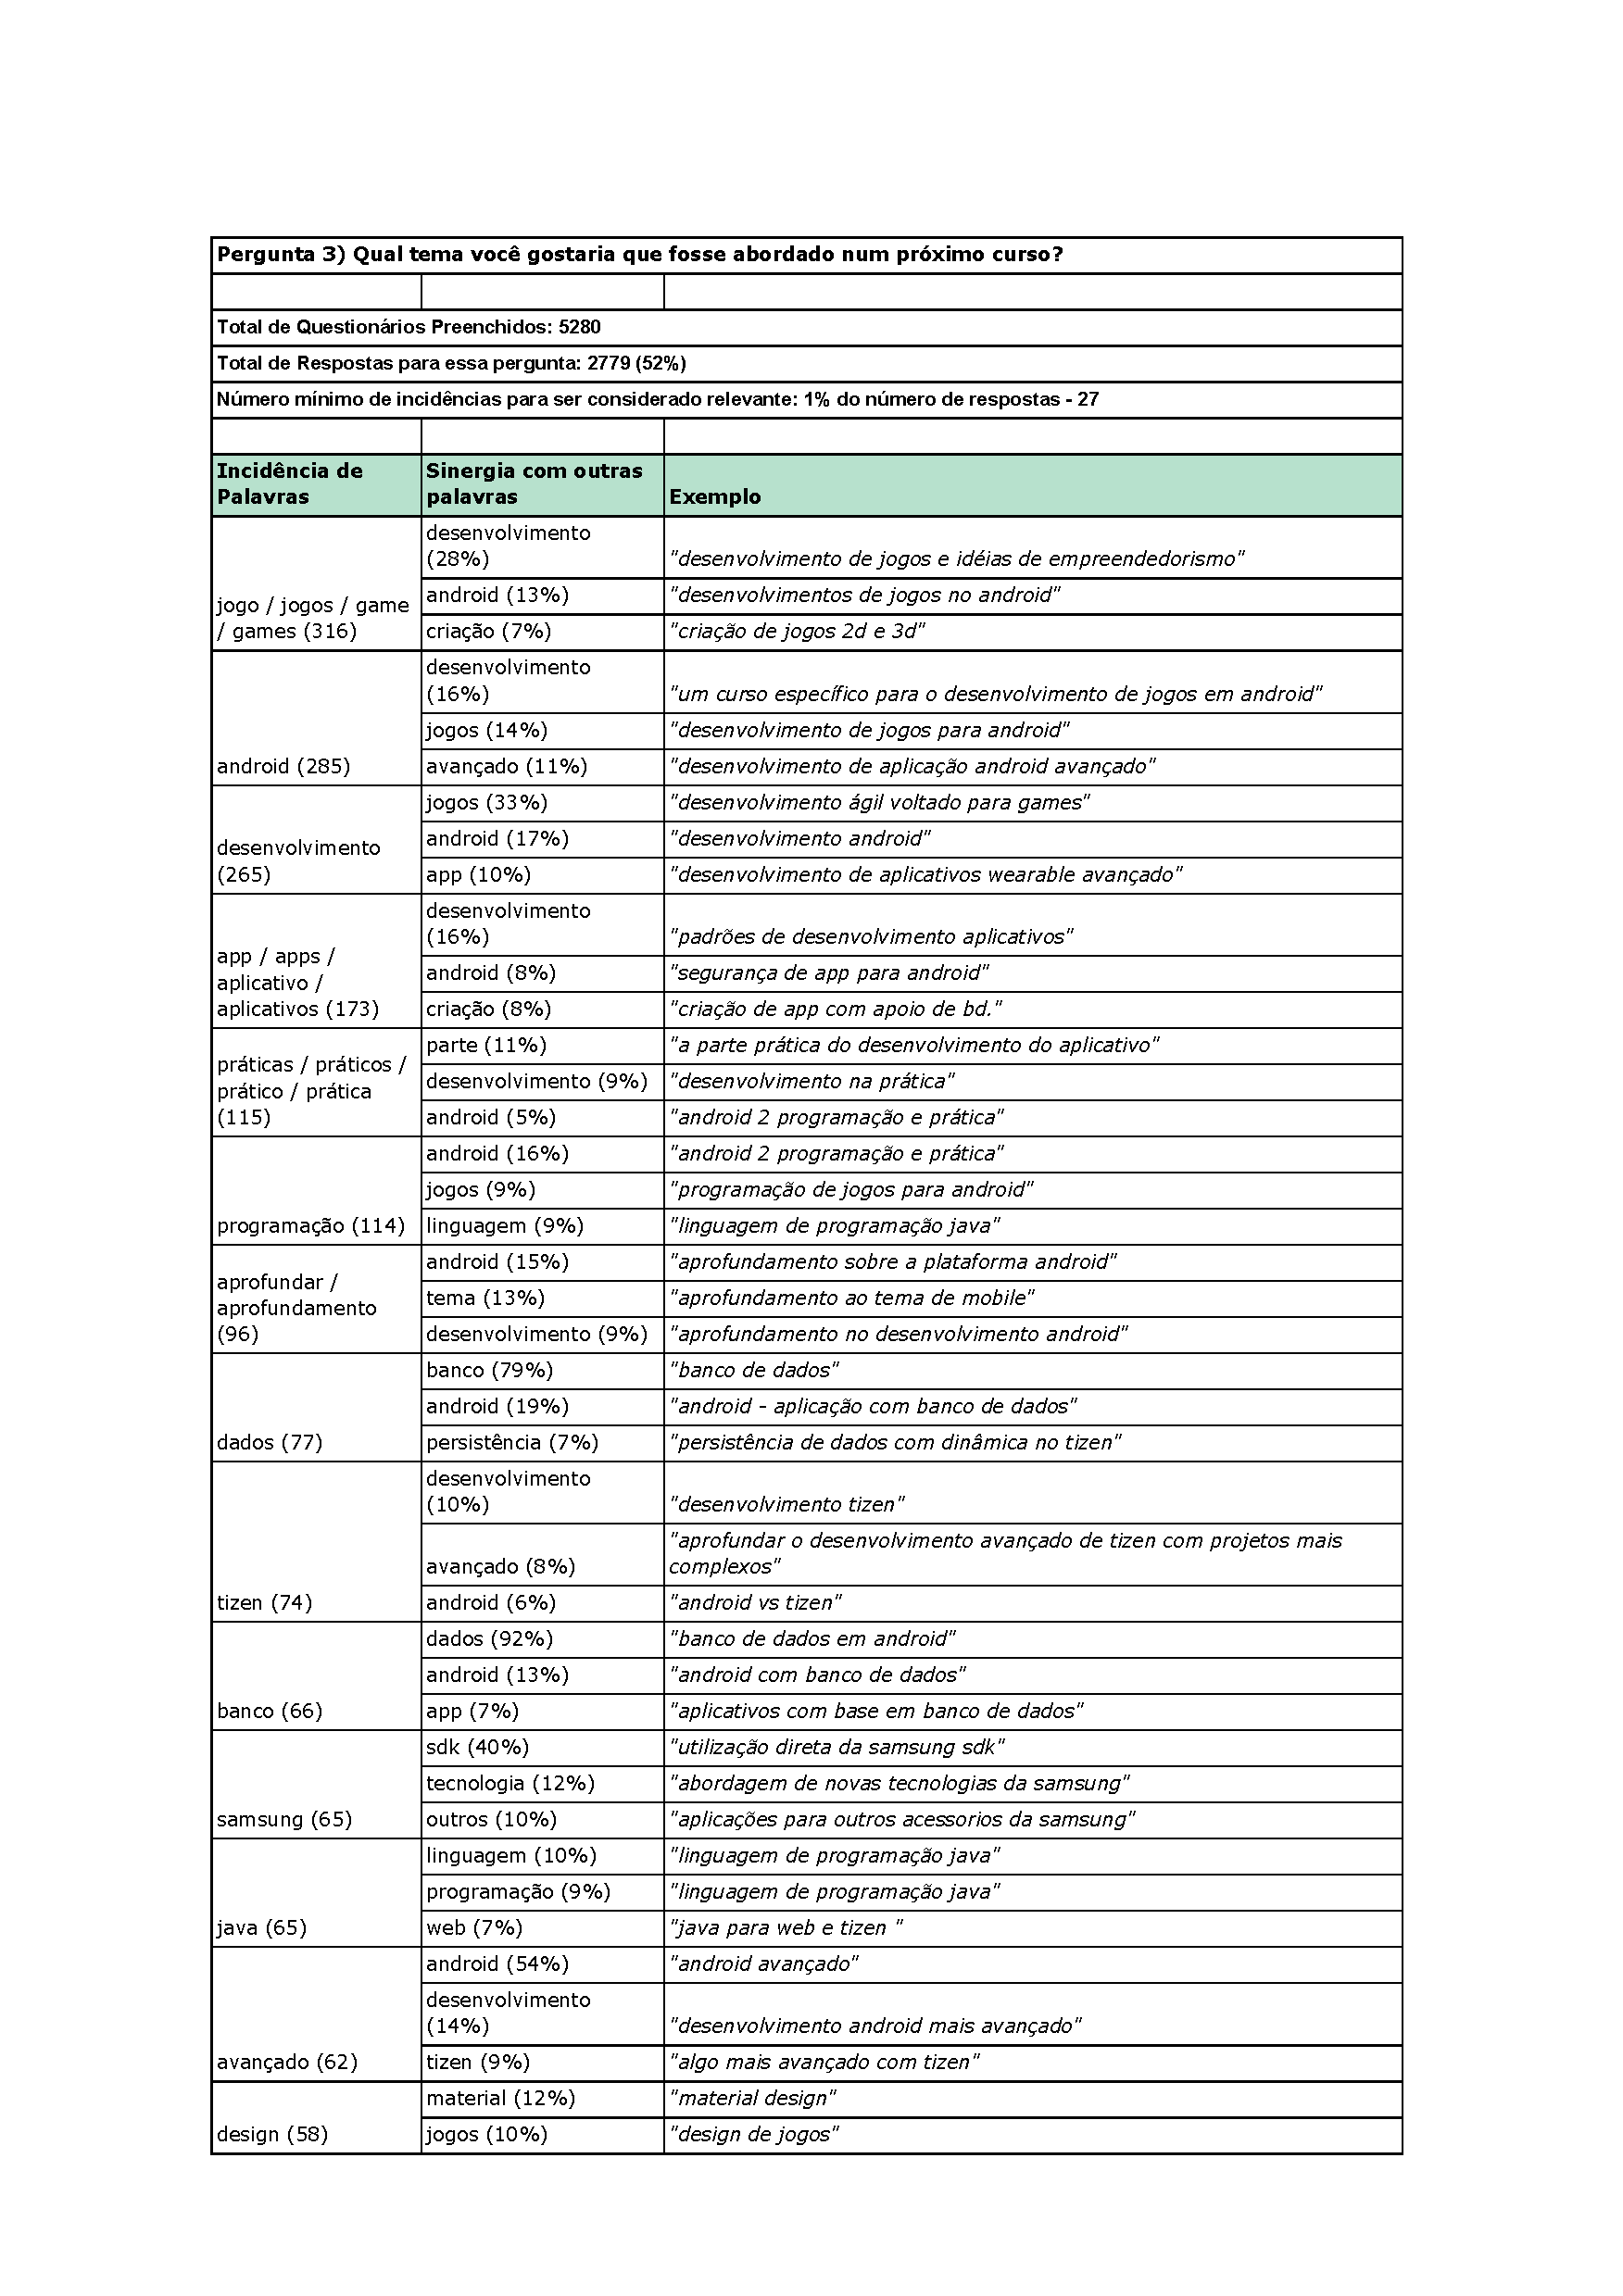
\includepdf[pages=-, pagecommand={}]{Pergunta3.pdf}

\subsubsection*{Categorização e sub-categorização - \textit{Novidades}}

Em primeira instância, é possível visualizar uma grande demanda de alunos por aulas específicas para o desenvolvimento de jogos. É de grande relevância que esta questão é a de escopo mais aberto das três, portanto a grande recorrência do termo 'jogo' nesse contexto é bastante relevante. Além de jogos, existe uma demanda pela aplicação de android em outros casos de uso, como aplicativos ou uma exploração mais avançada do sistema operacional. 

Em menor volume porém com uma maior gama de opções, existe uma demanda por uma exploração de bancos de dados, tizen, maior exploração do sdk da samsung e outras tecnologias, linguagem de desenvolvimento java, design e user experience, desenvolvimento web, web services, e unity. 

\begin{figure}[h]
\caption{Análise do Ocean - Cursistas}
\centerline{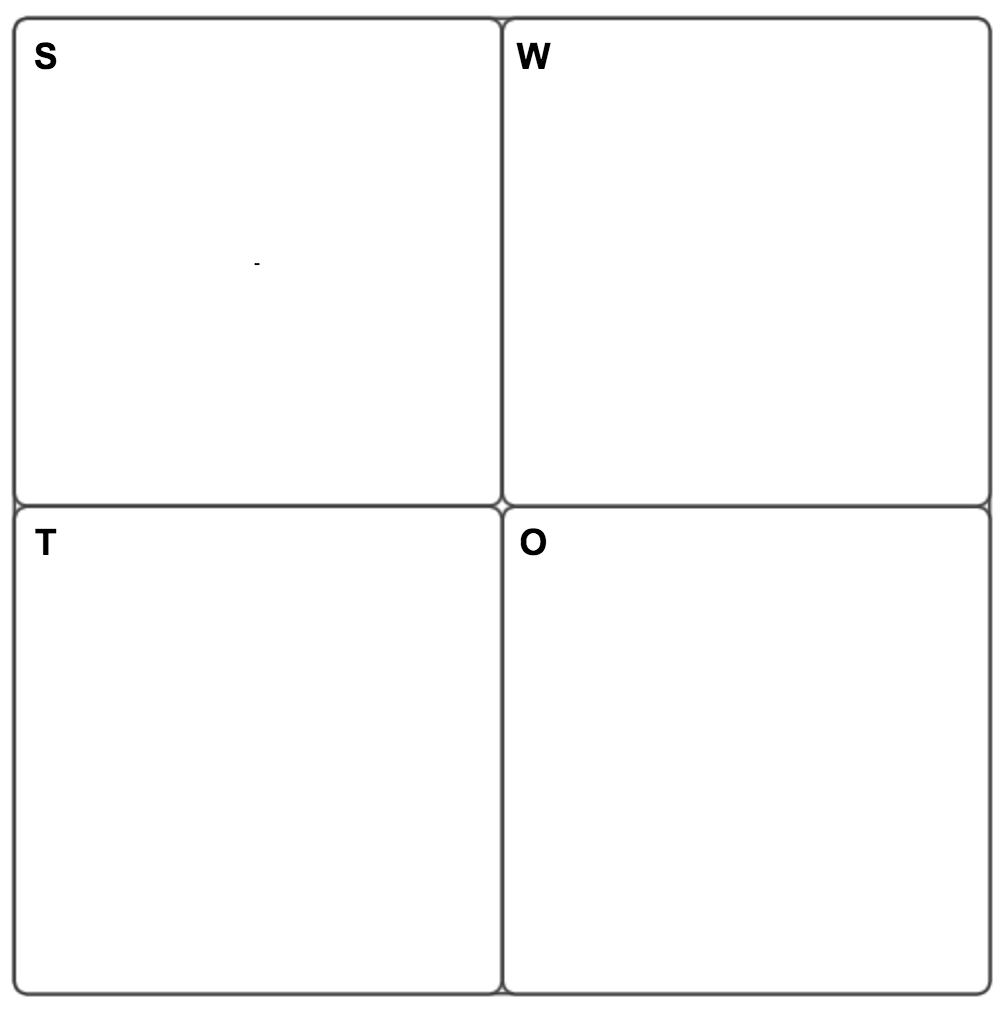
\includegraphics[scale=0.75]{img/generalswot}}
\label{fig:swotcursistas}
\caption* {Fonte: Elaborado pelo próprio autor}
\end{figure}